\chapter{Support Vector Machines (Intuition)}
\label{chap:svm_intuition}

\section{Introduction}
Logistic Regression is great, but it has a flaw: it cares only about being \textit{Right}.
If a point is classified correctly (even by a hair's breadth), Logistic Regression is happy.
**SVM** cares about being \textit{Confident}. It wants to be Right, and it wants a \textbf{Gap}.

\section{The "Widest Street" Analogy}
Imagine you are a city planner trying to build a new road (Decision Boundary) to separate the Red City from the Blue City.
\begin{itemize}
    \item You don't just want a thin line. You want a wide highway.
    \item The wider the highway (Margin), the safer the separation.
    \item The road edges can touch the houses, but cannot go \textit{through} them.
\end{itemize}

\begin{figure}[htbp]
\centering
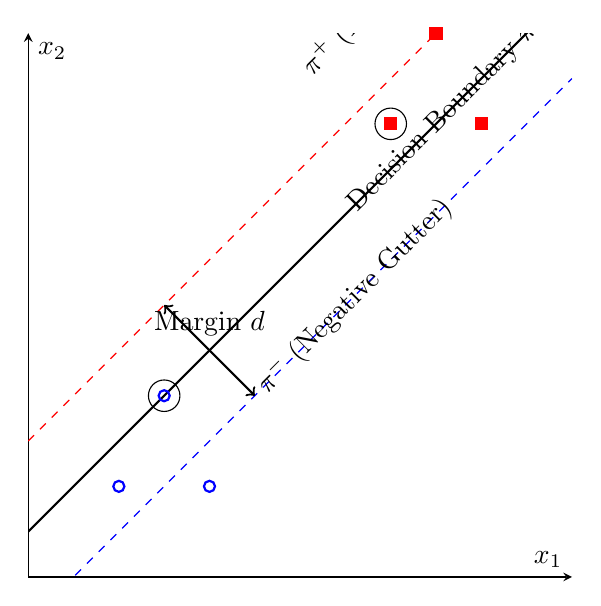
\begin{tikzpicture}
    \begin{axis}[
        xlabel={$x_1$}, ylabel={$x_2$},
        axis lines=middle,
        xmin=0, xmax=6, ymin=0, ymax=6,
        width=0.7\textwidth, height=0.7\textwidth,
        ticks=none
    ]
    % Data Points
    \addplot[only marks, mark=o, color=blue, thick] coordinates {(1,1) (2,1) (1.5,2)};
    \addplot[only marks, mark=square*, color=red, thick] coordinates {(4,5) (5,5) (4.5,6)};
    
    % Support Vectors (Circle them)
    \draw[black, thin] (axis cs:1.5,2) circle(0.2cm);
    \draw[black, thin] (axis cs:4,5) circle(0.2cm);
    
    % Hyperplane (Solid)
    \addplot[domain=0:6, color=black, thick] {x + 0.5};
    \node[right, rotate=45] at (axis cs:3.5, 4) {Decision Boundary $\pi$};
    
    % Margins (Dashed)
    \addplot[domain=0:6, color=blue, dashed] {x + 0.5 - 1.0}; % Shifted down
    \node[right, rotate=45] at (axis cs:2.5, 2) {$\pi^-$ (Negative Gutter)};
    
    \addplot[domain=0:6, color=red, dashed] {x + 0.5 + 1.0}; % Shifted up
    \node[right, rotate=45] at (axis cs:3, 5.5) {$\pi^+$ (Positive Gutter)};
    
    % Margin Arrow
    \draw[<->, thick] (axis cs:2.5, 2) -- (axis cs:1.5, 3);
    \node at (axis cs:2, 2.8) {Margin $d$};
    
    \end{axis}
\end{tikzpicture}
\caption{The Street (Margin). The algorithm pushes the dashed lines as far apart as possible until they hit the data points.}
\label{fig:svm_margin}
\end{figure}

\section{Core Terminology}
This geometry gives rise to three key definitions.

\begin{definition}
\textbf{Hyperplane ($\pi$)}: The decision boundary decision surface. In 2D, it is a line ($w^T x + b = 0$). Ideally, it lies exactly in the middle of the street.
\end{definition}

\begin{definition}
\textbf{Margin ($d$)}: The perpendicular distance between the two marginal planes (the "gutters"). SVM's goal is to \textbf{Maximize} this distance.
\end{definition}

\begin{definition}
\textbf{Support Vectors}: The specific data points that lie exactly on the edge of the margin. They "support" or "hold" the street in place.
\end{definition}

\textbf{Why is this called ``Support Vector Machine''?}
\\ Because the entire model is defined \textit{only} by these Support Vectors.
\\ If you delete the 99\% of data points that are far away from the road, the road does not move. The non-support vectors are mathematically irrelevant. This makes SVM distinct from Logistic Regression (which is affected by all points).

\section{Implementation in Python}
\begin{lstlisting}[language=Python, caption=Basic SVM Classifier]
from sklearn.svm import SVC
from sklearn.datasets import make_blobs
from sklearn.model_selection import train_test_split
from sklearn.preprocessing import StandardScaler

# Generate sample data
X, y = make_blobs(n_samples=100, centers=2, random_state=42)

# Scale features (important for SVM)
scaler = StandardScaler()
X_scaled = scaler.fit_transform(X)

# Train SVM
svm = SVC(kernel='linear', C=1.0)
svm.fit(X_scaled, y)

print(f"Number of Support Vectors: {len(svm.support_vectors_)}")
print(f"Accuracy: {svm.score(X_scaled, y):.2f}")
\end{lstlisting}

\section{HOTS: Interview Questions}
\textbf{Q1: Why is SVM called a ``Maximum Margin Classifier''?}
\begin{itemize}
    \item Because SVM explicitly tries to find the hyperplane that maximizes the distance (margin) between the decision boundary and the nearest data points (support vectors).
\end{itemize}

\textbf{Q2: How does SVM differ from Logistic Regression?}
\begin{itemize}
    \item Logistic Regression minimizes log-loss and is affected by all data points.
    \item SVM maximizes margin and is affected only by support vectors.
    \item SVM uses Hinge Loss, Logistic Regression uses Log Loss.
\end{itemize}

% ========================================
% SECTION: QUICK REFERENCE
% ========================================
\section{Quick Reference Card}

\begin{center}
\fbox{\parbox{0.9\textwidth}{
\textbf{SVM INTUITION - CHEAT SHEET}
\vspace{0.3cm}

\textbf{Core Idea}: Find the ``widest street'' (maximum margin) separating classes

\textbf{Key Components}:
\begin{itemize}
    \item \textbf{Hyperplane}: Decision boundary $w^Tx + b = 0$
    \item \textbf{Margin}: Distance between boundary and nearest points
    \item \textbf{Support Vectors}: Points on the margin edge (the VIPs)
\end{itemize}

\textbf{Margin Width}: $\frac{2}{||w||}$ (maximize by minimizing $||w||$)

\textbf{SVM vs Logistic Regression}:
\begin{center}
\begin{tabular}{|l|l|l|}
\hline
& \textbf{SVM} & \textbf{LogReg} \\ \hline
Loss & Hinge & Log \\ \hline
Points Used & Support Vectors only & All \\ \hline
Goal & Max Margin & Min Log-Loss \\ \hline
\end{tabular}
\end{center}

\textbf{Sklearn}: \texttt{SVC(kernel='linear', C=1.0)}

\textbf{Interview Gold}:
\begin{itemize}
    \item Only support vectors affect the decision
    \item MUST scale features (distance-based)
    \item C controls margin width vs errors tradeoff
\end{itemize}
}}
